\flushbottom

% CONTINUE: define neighborhoods, balls, etc.


%============================================================================
%============================================================================
\chapter{Sets and Functions}




%=============================================================================
\section{Sets}


\paragraph{Definition.}
A \textit{set} is a collection of objects.  We call the objects, 
\index{set}
\textit{elements}.   A set is denoted by listing the elements between
\index{elements!of a set}
braces.  For example: $\{\e, \imath, \pi, 1\}$ is the set of the integer $1$, the 
pure imaginary number $\imath = \sqrt{-1}$ and the transcendental numbers
$\e = 2.7182818\ldots$ and $\pi = 3.1415926\ldots$.   
For elements of a set, we do not count multiplicities.  We regard the set
$\{1, 2, 2, 3, 3, 3\}$ as identical to the set $\{1,2,3\}$.
Order is not significant in sets.  The set $\{1,2,3\}$ is equivalent to 
$\{3,2,1\}$.

In enumerating the elements of a set, we use ellipses to indicate 
patterns.  We denote the set of positive integers as $\{1, 2, 3, \ldots\}$.
We also denote sets with the notation $\{x | \mathrm{conditions on}\ x \}$
for sets that are more easily described than enumerated.  This is read as
``the set of elements $x$ such that \ldots''.  
$x \in S$ is the notation for ``$x$ is an element of the set $S$.''
To express the opposite we have $x \not\in S$ for 
``$x$ is not an element of the set $S$.''



\paragraph{Examples.}
We have notations for denoting some of the commonly encountered sets.
\begin{itemize}
\item
$\emptyset = \{\}$ is the \textit{empty set}, the set containing no elements.
\index{empty set}
\item
$\mathbb{Z} = \{\ldots, -3, -2, -1, 0, 1, 2, 3 \ldots\}$ is the set of 
\textit{integers}.  (Z is for ``Zahlen'', the German word for ``number''.)
\index{integers!set of}
\item
$\mathbb{Q} = \{ p / q | p,q \in \mathbb{Z}, q \neq 0 \}$ is the set of 
\textit{rational numbers}.  (Q is for quotient.)
\index{rational numbers!set of}
\footnote{
  Note that with this description, we enumerate each rational number an 
  infinite number of times.  For example: $1/2 = 2/4 = 3/6 = (-1)/(-2) = \cdots$.
  This does not pose a problem as we do not count multiplicities.
}
\item
%% CONTINUE: Define this properly.
$\mathbb{R} = \{ x | x = a_1 a_2 \cdots a_n.b_1 b_2 \cdots \}$ is the set
of \textit{real numbers}, i.e. the set of numbers with decimal expansions.
\footnote{Guess what R is for.}
\index{real numbers!set of}
\item
$\mathbb{C} = \{ a + \imath b | a,b \in \mathbb{R}, \imath^2 = -1 \}$ is the set of 
\textit{complex numbers}.  $\imath$ is the square root of $-1$.  
(If you haven't seen complex numbers before, don't dismay.  
We'll cover them later.)
\index{complex numbers!set of}
\item
$\mathbb{Z}^+$, $\mathbb{Q}^+$ and $\mathbb{R}^+$ are the sets of 
positive integers, rationals and reals, respectively.  For example,
$\mathbb{Z}^+ = \{1, 2, 3, \ldots\}$.  We use a $-$ superscript to denote 
the sets of negative numbers.
\item
$\mathbb{Z}^{0+}$, $\mathbb{Q}^{0+}$ and $\mathbb{R}^{0+}$ are the sets of 
non-negative integers, rationals and reals, respectively.  For example,
$\mathbb{Z}^{0+} = \{0, 1, 2, \ldots\}$.
\item
$(a \ldots b)$ denotes an \textit{open interval} on the real axis.
$(a \ldots b) \equiv \{ x | x \in \mathbb{R}, a < x < b \}$
\index{open interval}
\index{interval!open}
\item
We use brackets to denote the \textit{closed interval}.
$[a .. b] \equiv \{ x | x \in \mathbb{R}, a \leq x \leq b \}$
\index{closed interval}
\index{interval!closed}
\end{itemize}



The \textit{cardinality} or \textit{order} of a set $S$ is denoted $|S|$.
\index{cardinality!of a set}
\index{order!of a set}
%% CONTINUE: Cover the cardinality of infinite sets.
For finite sets, the cardinality is the number of elements in the set.
The \textit{Cartesian product} of two sets is the set of ordered pairs:
\index{Cartesian product!of sets}
\[
X \times Y \equiv \{ (x,y) | x \in X, y \in Y \}.
\]
The Cartesian product of $n$ sets is the set of ordered n-tuples:
\[
X_1 \times X_2 \times \cdots \times X_n \equiv \{ (x_1,x_2,\ldots,x_n) | x_1 \in X_1, x_2 \in X_2, \ldots, x_n \in X_n \}.
\]


\paragraph{Equality.}
Two sets $S$ and $T$ are \textit{equal} if each element of $S$ is an element 
of $T$ and vice versa.  This is denoted, $S = T$.  Inequality is
$S \neq T$, of course.
$S$ is a \textit{subset}
\index{subset}
of $T$, $S \subseteq T$, if every element of $S$ is an element of $T$.
$S$ is a \textit{proper subset}
\index{subset!proper}
of $T$, $S \subset T$, if $S \subseteq T$ and $S \neq T$.
For example: The empty set is a subset of every set, $\emptyset \subseteq S$.
The rational numbers are a proper subset of the real numbers, 
$\mathbb{Q} \subset \mathbb{R}$.


\paragraph{Operations.}
The \textit{union} of two sets, $S \cup T$,  is the set whose elements are 
\index{union!of sets}
in either of the two sets.
The union of $n$ sets,
\[
\cup_{j=1}^n S_j \equiv S_1 \cup S_2 \cup \cdots \cup S_n
\]
is the set whose elements are in any of the sets $S_j$.
The \textit{intersection} of two sets, $S \cap T$,  is the set whose 
\index{intersection!of sets}
elements are in both of the two sets.  In other words, the intersection of
two sets in the set of elements that the two sets have in common.
The intersection of $n$ sets,
\[
\cap_{j=1}^n S_j \equiv S_1 \cap S_2 \cap \cdots \cap S_n
\]
is the set whose elements are in all of the sets $S_j$.
If two sets have no elements in common, $S \cap T = \emptyset$, then 
the sets are \textit{disjoint}.
\index{disjoint sets}
If $T \subseteq S$, then the \textit{difference} between $S$ and $T$,
\index{difference!of sets}
$S \setminus T$, is the set of elements in $S$ which are not in $T$.
\[
S \setminus T \equiv \{x | x \in S, x \not\in T \}
\]
The difference of sets is also denoted $S - T$.


\paragraph{Properties.}
The following properties are easily verified from the above definitions.
\begin{itemize}
\item 
$S \cup \emptyset = S$, $S \cap \emptyset = \emptyset$,
$S \setminus \emptyset = S$, $S \setminus S = \emptyset$. 
\item
Commutative.
$S \cup T = T \cup S$, $S \cap T = T \cap S$.
\item
Associative.
$(S \cup T) \cup U = S \cup (T \cup U) = S \cup T \cup U$,
$(S \cap T) \cap U = S \cap (T \cap U) = S \cap T \cap U$.
\item
Distributive.
$S \cup (T \cap U) = (S \cup T) \cap (S \cup U)$,
$S \cap (T \cup U) = (S \cap T) \cup (S \cap U)$.
\end{itemize}



% CONTINUE HERE




%=============================================================================
\section{Single Valued Functions}
\index{single-valued function}
\index{function!single-valued}

%% CONTINUE
%% Also introduce the ----jective terminology.

\paragraph{Single-Valued Functions.}
A \textit{single-valued function} or \textit{single-valued mapping}
is a mapping of the elements $x \in X$ 
into elements $y \in Y$.  This is expressed as $f : X \to Y$
or $X \stackrel{f}{\to} Y$.
If such a function is well-defined, then for each $x \in X$ there exists 
a unique element of $y$ such that $f(x) = y$.
The set $X$ is the \textit{domain} of the function, $Y$ is the 
\textit{codomain}, (not to be confused with the \textit{range}, which 
we introduce shortly).
\index{domain}
\index{codomain}
To denote the value of a function on a particular element we can use any 
of the notations: $f(x) = y$, $f : x \mapsto y$ or simply $x \mapsto y$.
$f$ is the \textit{identity map} on $X$ if $f(x) = x$ for all $x \in X$.
\index{identity map}

Let $f: X \to Y$.  The \textit{range} or \textit{image} of $f$ is
\index{range!of a mapping}
\index{image!of a mapping}
\[
f(X) = \{ y | y = f(x)\ \mathrm{for some}\ x \in X \}.
\]
The range is a subset of the codomain.  For each $Z \subseteq Y$, the 
\textit{inverse image} of $Z$ is defined:
\index{inverse image}
\[
f^{-1}(Z) \equiv \{ x \in X | f(x) = z\ \mathrm{for some}\ z \in Z \}.
\]

\paragraph{Examples.}
\begin{itemize}
\item
Finite polynomials, $f(x) = \sum_{k = 0}^n a_k x^k$, $a_k \in \mathbb{R}$, and the 
exponential function, $f(x) = \e^x$, are examples of single 
valued functions which map real numbers to real numbers.
\item
The \textit{greatest integer function}, $f(x) = \lfloor x\rfloor$, is a mapping from 
$\mathbb{R}$ to $\mathbb{Z}$.  $\lfloor x \rfloor$ is defined as the greatest integer less 
than or equal to $x$.  Likewise, the \textit{least integer function}, 
$f(x) = \lceil x \rceil$, is the least integer greater than or equal to $x$.
\index{greatest integer function}
\index{least integer function}
% CONTINUE HERE
\end{itemize}



\paragraph{The -jectives.}
A function is \textit{injective} if for each $x_1 \neq x_2$, 
$f(x_1) \neq f(x_2)$.
\index{function!injective}
In other words, distinct elements are mapped to distinct elements.
$f$ is \textit{surjective} if for each $y$ in the codomain,
\index{function!surjective}
there is an $x$ such that $y = f(x)$.  If a function is both injective and 
surjective, then it is \textit{bijective}.  A bijective function is also 
\index{function!bijective}
called a \textit{one-to-one mapping}.
\index{one-to-one mapping}


\paragraph{Examples.}
\begin{itemize}
\item
The exponential function $f(x) = \e^x$, considered as a mapping from
$\mathbb{R}$ to $\mathbb{R}^+$, is bijective, (a one-to-one mapping).
\item
$f(x)=x^2$ is a bijection from $\mathbb{R}^+$ to $\mathbb{R}^+$.  
$f$ is not injective from $\mathbb{R}$ to $\mathbb{R}^+$.  For each positive
$y$ in the range, there are two values of $x$ such that $y=x^2$.
\item
$f(x) = \sin x$ is not injective from $\mathbb{R}$ to $[-1..1]$.  
For each $y \in [-1..1]$ there exists an infinite number of values of 
$x$ such that $y = \sin x$.
\end{itemize}


\begin{figure}[h!]
\begin{center}
\includegraphics[width=0.8\textwidth]{algebra/sets/jectives}
\end{center}
\caption{Depictions of Injective, Surjective and Bijective Functions}
\label{jectives}
\end{figure}





% CONTINUE HERE
% Function composition, left and right inverses.





%=============================================================================
\section{Inverses and Multi-Valued Functions}
\index{inverse function}
\index{function!inverse of}
\index{multi-valued function}
\index{function!multi-valued}


If $y = f(x)$, then we can write $x = f^{-1}(y)$ where $f^{-1}$ is the inverse of 
$f$.  If $y = f(x)$ is a one-to-one function, then $f^{-1}(y)$ is also
a one-to-one function.  In this case, $x = f^{-1}(f(x)) = f(f^{-1}(x))$
for values of $x$ where both $f(x)$ and $f^{-1}(x)$ are defined.
For example $\ln x$, which maps $\mathbb{R}^+$ to $\mathbb{R}$ is 
the inverse of $\e^x$.  $x = \e^{\ln x} = \ln( \e^x )$ for all 
$x \in \mathbb{R}^+$.  (Note the $x \in \mathbb{R}^+$ ensures that 
$\ln x$ is defined.)

If $y = f(x)$ is a many-to-one function, then $x = f^{-1}(y)$ is a one-to-many
function.  $f^{-1}(y)$ is a multi-valued function.  We have
$x = f(f^{-1}(x))$ for values of $x$ where $f^{-1}(x)$ is defined, however 
$x \neq f^{-1}(f(x))$.  There are diagrams showing one-to-one, many-to-one
and one-to-many functions in Figure~\ref{tototo}.

\begin{figure}[h!]
\begin{center}
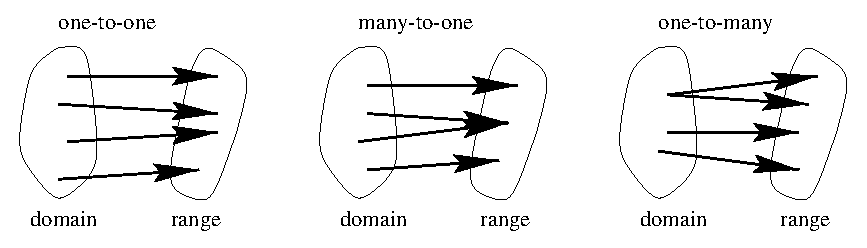
\includegraphics[width=0.8\textwidth]{algebra/sets/tototo}
\end{center}
\caption{Diagrams of One-To-One, Many-To-One and One-To-Many Functions}
\label{tototo}
\end{figure}






\begin{Example}
$y=x^2$ is a many-to-one function that has the inverse $x=y^{1/2}$.  For each 
positive $y$, there are two values of $x$ such that $x=y^{1/2}$.
$y = x^2$ and $y = x^{1/2}$ are graphed in Figure~\ref{yexsyesx}.
\begin{figure}[h!]
\begin{center}
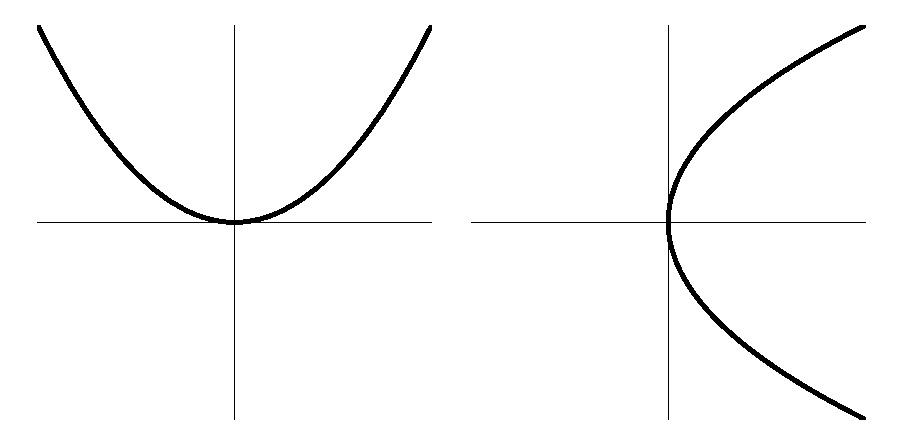
\includegraphics[width=0.4\textwidth]{algebra/sets/yexsyesx}
\end{center}
\caption{A many-to-one function and its multi-valued inverse.}
\label{yexsyesx}
\end{figure}
\end{Example}






We say that there are two \textit{branches}
\index{branches}
of $y=x^{1/2}$: the positive and the negative branch.  We denote the positive
branch as $y=\sqrt{x}$; the negative branch is $y=-\sqrt{x}$.  We call
$\sqrt{x}$ the \textit{principal branch}
\index{principal branch}
\index{branch!principal}
of $x^{1/2}$.  Note that $\sqrt{x}$ is a one-to-one function.
Finally, $x=(x^{1/2})^2$ since $(\pm \sqrt{x})^2  =x$, but
$x \neq (x^2)^{1/2}$ since $(x^2)^{1/2} = \pm x$.
$y = \sqrt{x}$ is graphed in Figure~\ref{yesqrtx}.

\begin{figure}[h!]
\begin{center}
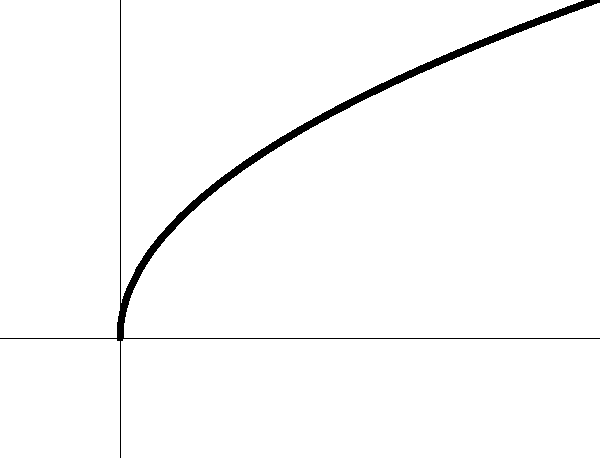
\includegraphics[width=0.3\textwidth]{algebra/sets/yesqrtx}
\end{center}
\caption{The positive branch of the square root.}
\label{yesqrtx}
\end{figure}



Now consider the many-to-one function $y=\sin x$.  The inverse is 
$x=\arcsin y$.  For each $y \in [-1..1]$ there are an infinite number
of values $x$ such that $x = \arcsin y$.
In Figure~\ref{yesxyeax} is a graph of $y = \sin x$ and a graph of a few 
branches of $y = \arcsin x$.

\begin{figure}[h!]
\begin{center}
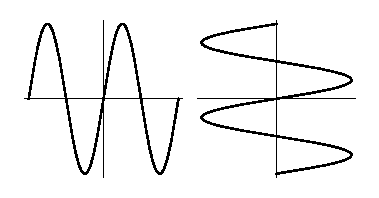
\includegraphics[width=0.4\textwidth]{algebra/sets/yesxyeax}
\end{center}
\caption{The sine and the arcsine.}
\label{yesxyeax}
\end{figure}






\begin{Example}
$\arcsin x$ has an infinite number of branches.  We will denote the
principal branch by $\Arcsin x$ which maps $[-1..1]$ to 
$\left[ -\frac{\pi}{2}.. \frac{\pi}{2} \right]$.
Note that $x = \sin(\arcsin x)$, but $x \neq \arcsin( \sin x )$.
$y = \Arcsin x$ in Figure~\ref{yepbax}.
\begin{figure}[h!]
\begin{center}
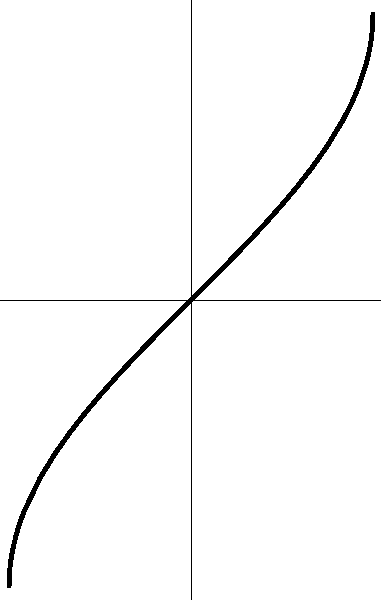
\includegraphics[width=0.2\textwidth]{algebra/sets/yepbax}
\end{center}
\caption{The principal branch of the arcsine.}
\label{yepbax}
\end{figure}
\end{Example}







\begin{Example}
Consider $1^{1/3}$.
Since $x^3$ is a one-to-one function, $x^{1/3}$ is a single-valued function.
(See Figure~\ref{yexcyecx}.) $1^{1/3} = 1$.
\begin{figure}[h!]
\begin{center}
\includegraphics[width=0.4\textwidth]{algebra/sets/yexcyecx}
\end{center}
\caption{A one-to-one function and its inverse.}
\label{yexcyecx}
\end{figure}
\end{Example}







\begin{Example}
Consider $\arccos(1/2)$.  $\cos x$ and a portion of $\arccos x$ are 
graphed in Figure~\ref{yecxyeax}.
The equation $\cos x = 1/2$ has the two solutions $x = \pm \pi / 3$ in the range
$x \in (-\pi..\pi]$.  We use the periodicity of the cosine, 
$\cos(x + 2 \pi) = \cos x$, to find the remaining solutions.
\[
\arccos(1/2) = \{ \pm \pi / 3 + 2 n \pi \}, \quad n \in \mathbb{Z}.
\]

\begin{figure}[h!]
\begin{center}
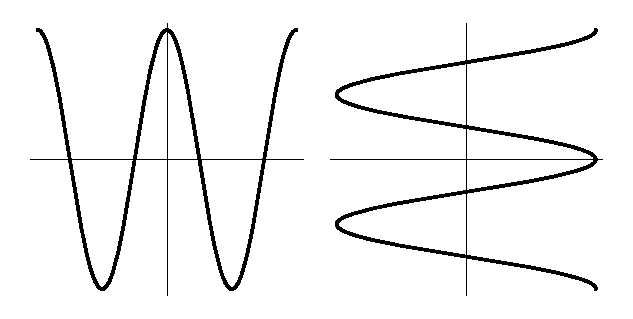
\includegraphics[width=0.4\textwidth]{algebra/sets/yecxyeax}
\end{center}
\caption{The cosine and the arccosine.}
\label{yecxyeax}
\end{figure}
\end{Example}











%=============================================================================
\section{Transforming Equations}

Consider the equation $g(x) = h(x)$ and the single-valued function $f(x)$.
A particular value of $x$
is a solution of the equation if substituting that value into the equation
results in an identity.  In determining the solutions of an equation, we 
often apply functions to each side of the equation in order to simplify
its form.  
We apply the function to obtain a second equation, $f(g(x)) = f(h(x))$.
If $x = \xi$ is a solution of the former equation, (let $\psi = g(\xi) = h(\xi)$), 
then it is necessarily a solution of latter.  This is because
$f(g(\xi)) = f(h(\xi))$ reduces to the identity $f(\psi) = f(\psi)$.
If $f(x)$ is bijective, then the converse is true: any solution of the 
latter equation is a solution of the former equation.  Suppose that
$x = \xi$ is a solution of the latter, $f(g(\xi)) = f(h(\xi))$.  That
$f(x)$ is a one-to-one mapping implies that $g(\xi) = h(\xi)$.  Thus $x = \xi$
is a solution of the former equation.

It is always safe to apply a one-to-one, (bijective), function to an equation, 
(provided it is defined for that
domain).  For example, we can apply $f(x) = x^3$ or $f(x) = \e^x$,
considered as mappings on $\mathbb{R}$, to the 
equation $x = 1$.  The equations $x^3 = 1$ and $\e^x = e$ each have the unique
solution $x = 1$ for $x \in \mathbb{R}$.


In general, we must take care in applying functions to equations.
If we apply a many-to-one function, we may introduce spurious
solutions.  Applying $f(x) = x^2$ to the equation
$x = \frac{\pi}{2}$ results in $x^2 = \frac{\pi^2}{4}$, which has the two solutions,
$x = \{ \pm \frac{\pi}{2} \}$.
Applying $f(x) = \sin x$ results in $x^2 = \frac{\pi^2}{4}$, which has 
an infinite number of solutions,
$x = \{ \frac{\pi}{2} + 2 n \pi \,|\, n \in \mathbb{Z} \}$.




We do not generally apply a one-to-many, (multi-valued), function to 
both sides of an equation as this rarely is useful.  Rather, we typically
use the definition of the inverse function.  Consider the equation
\[
\sin^2 x = 1.
\]
Applying the function $f(x) = x^{1/2}$ to the equation would not get us 
anywhere.
\[
\left( \sin^2 x \right)^{1/2} = 1^{1/2}
\]
Since $(\sin^2 x)^{1/2} \neq \sin x$, we cannot simplify the 
left side of the equation.  Instead we could use the definition of
$f(x) = x^{1/2}$ as the inverse of the $x^2$ function to obtain
\[
\sin x = 1^{1/2} = \pm 1.
\]
Now note that we should not just apply $\arcsin$ to both sides of the equation
as $\arcsin(\sin x) \neq x$.
Instead we use the definition of $\arcsin$ as the inverse of $\sin$.
\[
x = \arcsin( \pm 1)
\]
$x = \arcsin(1)$ has the solutions $x = \pi/2 + 2 n \pi$ and $x = \arcsin(-1)$
has the solutions $x = -\pi/2 + 2 n \pi$.  We enumerate the solutions.
\[
x = \left\{ \frac{\pi}{2} + n \pi \,|\, \quad n \in \mathbb{Z} \right\}
\]







%% CONTINUE
%% Add a section (from the notebook) on visualizing functions.



\raggedbottom
%============================================================================
\exercises{
\pagebreak
\flushbottom
\section{Exercises}

%-----------------------------------------------------------------------------
%\begin{large}
%\noindent
%\textbf{}
%\end{large}




\begin{Exercise}
\label{exercise area proportional square of diameter}
The area of a circle is directly proportional to the square of its diameter.
What is the constant of proportionality?

\hintsolution{area proportional square of diameter}
\end{Exercise}








\begin{Exercise}
\label{exercise x1y2=x21y24}
Consider the equation
\[
\frac{x+1}{y-2} = \frac{x^2 - 1}{y^2 - 4}.
\]
\begin{enumerate}
\item
  Why might one think that this is the equation of a line?
\item
  Graph the solutions of the equation to demonstrate that it is not the 
  equation of a line.
\end{enumerate}

\hintsolution{x1y2=x21y24}
\end{Exercise}



\begin{Exercise}
\label{exercise domain range 1x22}
Consider the function of a real variable,
\[
f(x) = \frac{1}{x^2 + 2}.
\]
What is the domain and range of the function?

\hintsolution{domain range 1x22}
\end{Exercise}





\begin{Exercise}
\label{exercise fahrenheit celcius}
The temperature measured in degrees Celsius 
\footnote{
  Originally, it was called degrees \textit{Centigrade}.  
  \textit{centi} because there are 100 degrees between the two 
  calibration points.  It is now called degrees Celsius in honor of the 
  inventor.
}
is linearly related to 
the temperature measured in degrees Fahrenheit
\footnote{
  The Fahrenheit scale, named for Daniel Fahrenheit,
  was originally calibrated with the freezing point of 
  salt-saturated water to be $0^\circ $.  Later, the calibration points 
  became the freezing point of water, $32^\circ$, and body temperature,
  $96^\circ$.  With this method, there are 64 divisions between the calibration
  points.  Finally, the upper calibration point was changed to the boiling
  point of water at $212^\circ$.  This gave 180 divisions, (the number of 
  degrees in a half circle), between the two calibration points.
}.
Water freezes at $0^\circ\ C = 32^\circ\ F$ and boils at 
$100^\circ\ C = 212^\circ\ F$.  Write the temperature in degrees Celsius
as a function of degrees Fahrenheit.

\hintsolution{fahrenheit celcius}
\end{Exercise}








\begin{Exercise}
\label{exercise xsinx transform}
Consider the function graphed in Figure~\ref{figure xsinx}.
Sketch graphs of $f(-x)$, $f(x+3)$, $f(3-x)+2$, and $f^{-1}(x)$.
You may use the blank grids in Figure~\ref{figure xsinx blank grids}.

\begin{figure}[h!]
\begin{center}
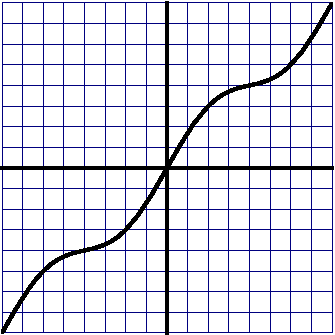
\includegraphics[width=0.4\textwidth]{algebra/sets/xsinx}
\end{center}
\caption{Graph of the function.}
\label{figure xsinx}
\end{figure}

\begin{figure}[tbp]
\begin{center}
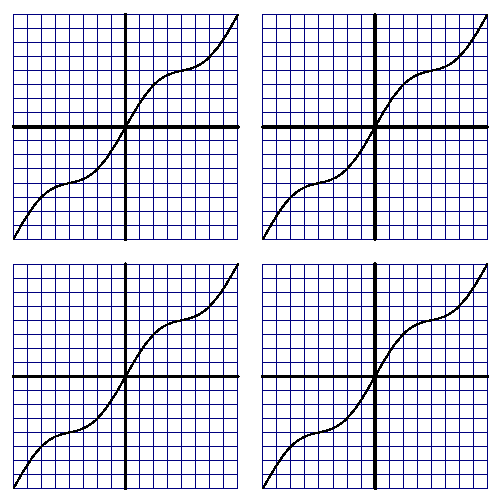
\includegraphics[width=0.7\textwidth]{algebra/sets/xsinx_blank}
\end{center}
\caption{Blank grids.}
\label{figure xsinx blank grids}
\end{figure}

\hintsolution{xsinx transform}
\end{Exercise}





\begin{Exercise}
\label{exercise geometric growth bacteria}
A culture of bacteria grows at the rate of $10\%$ per minute.  At 6:00 pm 
there are 1 billion bacteria.  How many bacteria are there at 7:00 pm?
How many were there at 3:00 pm?

\hintsolution{geometric growth bacteria}
\end{Exercise}





\begin{Exercise}
\label{exercise rational quadratic}
The graph in Figure~\ref{figure 2x2x21} shows an even function
$f(x) = p(x) / q(x)$ where $p(x)$ and $q(x)$ are rational quadratic 
polynomials.  Give possible formulas for $p(x)$ and $q(x)$.
\begin{figure}[tpb]
\begin{center}
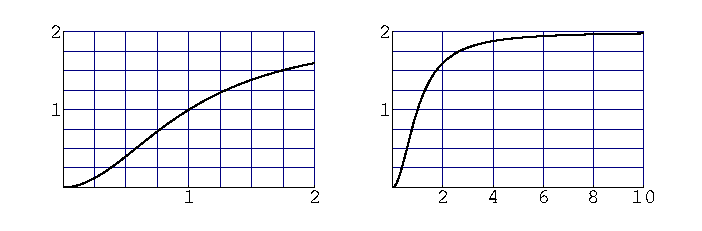
\includegraphics[width=0.8\textwidth]{algebra/sets/2x2x21}
\end{center}
\caption{Plots of a ratio of quadratic polynomials.}
\label{figure 2x2x21}
\end{figure}

\hintsolution{rational quadratic}
\end{Exercise}







\begin{Exercise}
\label{exercise polynomial 100}
Find a polynomial of degree 100 which is zero only at $x = -2, 1, \pi$ and
is non-negative.

\hintsolution{polynomial 100}
\end{Exercise}








\raggedbottom
}
%============================================================================
\hints{
\pagebreak
\flushbottom
\section{Hints}

%-----------------------------------------------------------------------------
%\begin{large}
%\noindent
%\textbf{}
%\end{large}


\begin{Hint}
\label{hint area proportional square of diameter}
$\mathrm{area} = \mathrm{constant} \times \mathrm{diameter}^2$.
\end{Hint}



\begin{Hint}
\label{hint x1y2=x21y24}
A pair $(x,y)$ is a solution of the equation if it make the equation 
an identity.
\end{Hint}


\begin{Hint}
\label{hint domain range 1x22}
The domain is the subset of $\mathbb{R}$ on which the function is defined.
\end{Hint}




\begin{Hint}
\label{hint fahrenheit celcius}
Find the slope and $x$-intercept of the line.
\end{Hint}




\begin{Hint}
\label{hint xsinx transform}
The inverse of the function is the reflection of the function across
the line $y = x$.
\end{Hint}



\begin{Hint}
\label{hint geometric growth bacteria}
The formula for geometric growth/decay is $x(t) = x_0 r^t$, where $r$ is 
the rate.
\end{Hint}



\begin{Hint}
\label{hint rational quadratic}
Note that $p(x)$ and $q(x)$ appear as a ratio, they are determined only up to
a multiplicative constant.  We may take the leading coefficient of $q(x)$ to
be unity.
\[
f(x) = \frac{p(x)}{q(x)} = \frac{a x^2 + b x + c}{x^2 + \beta x + \chi}
\]
Use the properties of the function to solve for the unknown parameters.
\end{Hint}






\begin{Hint}
\label{hint polynomial 100}
Write the polynomial in factored form.
\end{Hint}













\raggedbottom
}
%============================================================================
\solutions{
\pagebreak
\flushbottom
\section{Solutions}

%-----------------------------------------------------------------------------
%\begin{large}
%\noindent
%\textbf{}
%\end{large}





\begin{Solution}
\label{solution area proportional square of diameter}
\begin{gather*}
  \mathrm{area} = \pi \times \mathrm{radius}^2
  \\
  \mathrm{area} = \frac{\pi}{4} \times \mathrm{diameter}^2
\end{gather*}
The constant of proportionality is $\frac{\pi}{4}$.
\end{Solution}







\begin{Solution}
\label{solution x1y2=x21y24}
\begin{enumerate}
\item
If we multiply the equation by $y^2 - 4$ and divide by $x + 1$, we obtain 
the equation of a line.
\[
y + 2 = x - 1
\]
\item
We factor the quadratics on the right side of the equation.
\[
\frac{x+1}{y-2} = \frac{(x+1)(x-1)}{(y-2)(y+2)}.
\]
We note that one or both sides of the equation are undefined at $y = \pm 2$ 
because of division by zero.  There are no solutions for these two values of
$y$ and we assume from this point that $y \neq \pm 2$.  We multiply by 
$(y-2)(y+2)$.
\[
(x+1)(y+2) = (x+1)(x-1)
\]

For $x = -1$, the equation becomes the identity $0 = 0$.  Now we consider 
$x \neq -1$.  We divide by $x + 1$ to obtain the equation of a line.
\begin{gather*}
  y+2 = x-1
  \\
  y = x - 3
\end{gather*}
Now we collect the solutions we have found.
\[
\boxed{
  \{ (-1,y) : y \neq \pm 2 \} \cup \{ (x,x-3) : x \neq 1,5 \} 
  }
\]
The solutions are depicted in Figure~/ref{fig not a line}.

\begin{figure}[h!]
\begin{center}
\includegraphics[width=0.4\textwidth]{algebra/sets/not_a_line}
\end{center}
\caption{The solution is not a line.}
\label{fig not a line}
\end{figure}

\end{enumerate}
\end{Solution}








\begin{Solution}
\label{solution domain range 1x22}
The denominator is nonzero for all $x \in \mathbb{R}$.  Since we don't have 
any division by zero problems, the domain of the function is $\mathbb{R}$.
For $x \in \mathbb{R}$, 
\[
0 < \frac{1}{x^2 + 2} \leq 2.
\]
Consider 
\begin{equation}
  \label{eqn y = 1x22}
  y = \frac{1}{x^2 + 2}.
\end{equation}
For any $y \in (0 \ldots 1/2]$, there is at least one value of $x$ that satisfies 
Equation~\ref{eqn y = 1x22}.
\begin{gather*}
  x^2 + 2 = \frac{1}{y}
  \\
  x = \pm \sqrt{ \frac{1}{y} - 2 }
\end{gather*}
Thus the range of the function is $(0 \ldots 1/2]$
\end{Solution}






\begin{Solution}
\label{solution fahrenheit celcius}
Let $c$ denote degrees Celsius and $f$ denote degrees Fahrenheit.  The line
passes through the points $(f,c) = (32,0)$ and $(f,c) = (212,100)$.
The $x$-intercept is $f = 32$.  We calculate the slope of the line.
\[
\mathrm{slope} = \frac{100 - 0}{212 - 32} = \frac{100}{180} = \frac{5}{9}
\]
The relationship between fahrenheit and celcius is
\[
\boxed{
  c = \frac{5}{9} (f - 32).
  }
\]
\end{Solution}





\begin{Solution}
\label{solution xsinx transform}
We plot the various transformations of $f(x)$:
$f(-x)$, $f(x+3)$, $f(3-x)+2$, and $f^{-1}(x)$.
\begin{figure}[tbp]
\begin{center}
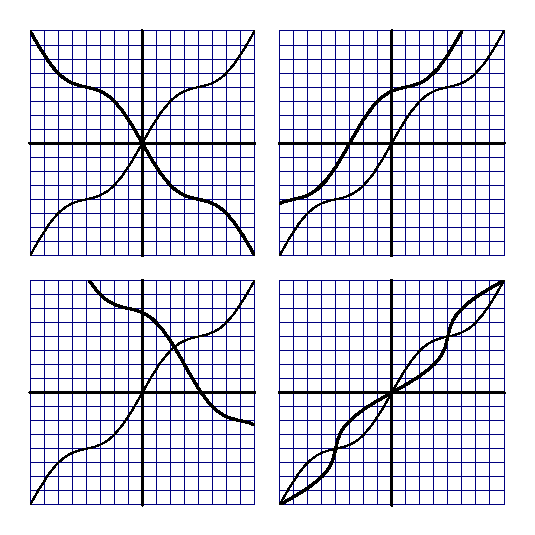
\includegraphics[width=0.7\textwidth]{algebra/sets/xsinx_transform}
\end{center}
\caption{Graphs of the transformations.}
\label{figure xsinx transform}
\end{figure}
\end{Solution}






\begin{Solution}
\label{solution geometric growth bacteria}
The formula for geometric growth/decay is $x(t) = x_0 r^t$, where $r$ is 
the rate.  Let $t = 0$ coincide with 6:00 pm.  We determine $x_0$.
\begin{gather*}
  x(0) = 10^9 = x_0 \left( \frac{11}{10} \right)^0 = x_0
  \\
  x_0 = 10^9
\end{gather*}
At 7:00 pm the number of bacteria is
\[
\boxed{
  10^9 \left( \frac{11}{10} \right)^{60} = \frac{11^{60}}{10^{51}} \approx 3.04 \times 10^{11}
  }
\]
At 3:00 pm the number of bacteria was
\[
\boxed{
  10^9 \left( \frac{11}{10} \right)^{-180} = \frac{10^{189}}{11^{180}} \approx 35.4
  }
\]
\end{Solution}











\begin{Solution}
\label{solution rational quadratic}
We write $p(x)$ and $q(x)$ as general quadratic polynomials.
\[
f(x) = \frac{p(x)}{q(x)} = \frac{a x^2 + b x + c}{\alpha x^2 + \beta x + \chi}
\]
We will use the properties of the function to solve for the unknown 
parameters.

Note that $p(x)$ and $q(x)$ appear as a ratio, they are determined only up to
a multiplicative constant.  We may take the leading coefficient of $q(x)$ to
be unity.
\[
f(x) = \frac{p(x)}{q(x)} = \frac{a x^2 + b x + c}{x^2 + \beta x + \chi}
\]
$f(x)$ has a second order zero at $x = 0$.  This means that $p(x)$ has a
second order zero there and that $\chi \neq 0$.
\[
f(x) = \frac{a x^2}{x^2 + \beta x + \chi}
\]
We note that $f(x) \to 2$ as $x \to \infty$.  This determines the parameter $a$.
\begin{align*}
  \lim_{x \to \infty} f(x)
  &= \lim_{x \to \infty} \frac{a x^2}{x^2 + \beta x + \chi}
  \\
  &= \lim_{x \to \infty} \frac{2 a x}{2 x + \beta}
  \\
  &= \lim_{x \to \infty} \frac{2 a}{2}
  \\
  &= a
\end{align*}
\[
f(x) = \frac{2 x^2}{x^2 + \beta x + \chi}
\]
Now we use the fact that $f(x)$ is even to conclude that $q(x)$ is even and
thus $\beta = 0$.
\[
f(x) = \frac{2 x^2}{x^2 + \chi}
\]
Finally, we use that $f(1) = 1$ to determine $\chi$.
\[
\boxed{
  f(x) = \frac{2 x^2}{x^2 + 1}
  }
\]
\end{Solution}








\begin{Solution}
\label{solution polynomial 100}
Consider the polynomial
\[
p(x) = (x + 2)^{40} (x - 1)^{30} (x - \pi)^{30}.
\]
It is of degree 100. Since the factors only vanish at $x = -2,1,\pi$, $p(x)$ 
only vanishes there.  Since factors are non-negative, the polynomial is 
non-negative.
\end{Solution}







\raggedbottom
}





